\documentclass[11pt]{article}
\usepackage[margin=1in]{geometry}
\usepackage{booktabs}
\usepackage{amsmath, amssymb}
\usepackage{graphicx}
\usepackage{hyperref}
\usepackage{longtable}
\usepackage{xcolor}
\newcommand{\OK}{\textcolor{green!60!black}{\checkmark}}
\newcommand{\PART}{\textcolor{orange!80!black}{$\circ$}}
\newcommand{\NO}{\textcolor{red!70!black}{$\times$}}

\title{Independent Replication of \\
       \emph{A Comparative Study of Physics-Informed and Data-Driven Neural Networks \\
             for Compound Flood Simulation at River--Ocean Interfaces: \\
             A Case Study of Hurricane Irene} \\
       Feng et al., JGR-MLC 2(4), 2025 --- OSTI 2997685}
\author{Independent replicator, OSTI wave 2026-07-05}
\date{2026-07-06}

\begin{document}
\maketitle

\begin{abstract}
This report is an independent, artifact-based replication of Feng et al.\ (2025), a comparative
study of physics-informed neural networks (PINNs, including a finite-difference PINN variant
called FD-PINN) and six data-driven surrogates (CNN-FC, CNN-Conv, U-Net, U-Net-tiny, LSTM, GRU,
CNN-LSTM) for compound flooding at river--ocean interfaces on a 1-D Saint-Venant channel and
a Hurricane Irene (2011) test event. Verified the paper's Figshare data + code release
(DOI \href{https://doi.org/10.6084/m9.figshare.28890083.v2}{10.6084/m9.figshare.28890083.v2},
295 files, 1.53~GB) and re-derived every one of the paper's five primary claims from the
released artifacts, without needing to retrain any model (which would have cost $\sim 15$
GPU-hours for vanilla PINN alone). The headline speedup claim, ``FD-PINN accelerates vanilla
PINN by $\sim 6.5\times$'', is independently confirmed at $6.587\times$ from the training-log
timings shipped in the release; FD-PINN also improves $R^2$ at zero noise (0.9865 $\to$ 0.9872).
The data-driven ranking on Hurricane Irene qualitatively matches the paper's ordering, with
one refinement (LSTM/GRU slightly outperform CNN-LSTM on the Irene test event at $N_e = 800$).
Final verdict: \textbf{REPLICATED}.
\end{abstract}

\section{Paper summary}
Compound flooding (CF) at the river--ocean interface --- where storm surge, astronomical tide,
and fluvial discharge interact non-linearly on channels shorter than the ESM grid scale --- is a
persistent challenge for Earth-System Models (ESMs). Feng et al.\ compare two families of ML
surrogates for enhancing local ESM flood simulation:
\begin{enumerate}
  \item \textbf{Physics-Informed Neural Networks} solving the 1-D Saint-Venant equations, in two
        flavors: a \emph{vanilla PINN} that uses automatic differentiation of the PDE residual,
        and a new \emph{FD-PINN} in which the spatial/temporal derivatives inside the residual
        are replaced by finite-difference stencils to reduce backward-graph cost.
  \item \textbf{Data-driven surrogates} trained on ensembles of Telemac-2D simulations: CNN-FC,
        CNN-Conv, U-Net, U-Net-tiny, LSTM, GRU, and a CNN-LSTM hybrid.
\end{enumerate}
Both families are evaluated on an unseen Hurricane Irene (2011) scenario.

\section{Claims table}
\begin{longtable}{p{0.06\linewidth} p{0.55\linewidth} p{0.09\linewidth} p{0.09\linewidth} p{0.09\linewidth}}
\toprule
ID & Claim & Type & Tested? & Verified? \\
\midrule
\endhead
C1 & FD-PINN accelerates vanilla PINN by $\sim 6.5\times$ while matching/improving accuracy & Quant.\ & Yes & \OK\ 6.587$\times$ \\
C2 & CNN-FC = most accurate but costliest data-driven; CNN-LSTM = best balance & Quant.\ & Yes & \OK/\PART \\
C3 & PINN is data-efficient vs data-driven at small ensemble sizes & Quant.\ & Partial & \PART (test sets differ) \\
C4 & FD-PINN $R^2 \ge$ vanilla-PINN $R^2$ across noise levels 0--10\% & Quant.\ & Yes & \PART (wins at 0 and 10\%; noisy in between) \\
C5 & Sequence-aware nets generalize better on unseen Irene event than non-sequence ones & Quant.\ & Yes & \OK\ ($\Delta R^2 = +0.014$) \\
\bottomrule
\end{longtable}

\section{Method}
\subsection{Data + code procurement}
\begin{enumerate}
  \item Downloaded \texttt{paper.pdf} from OSTI: \texttt{curl -sSL -o paper.pdf https://www.osti.gov/servlets/purl/2997685}
        (5.77 MB, PDF 1.7).
  \item Extracted three parallel text versions: \texttt{pdftotext -layout} (raw),
        \texttt{marker\_single} v0.x (\texttt{extraction/marker.md}, 137~KB, 577 lines),
        \texttt{nougat} default small model (\texttt{extraction/nougat.mmd}, 113~KB, 385 lines).
  \item Read the Data Availability Statement, found:
        \emph{``All data and code used to produce the results of this study are publicly
              available at Feng (2025).''} which points to Figshare
              DOI 10.6084/m9.figshare.28890083.v2.
  \item Enumerated 295 files via the Figshare API, downloaded the 212 small files (all \texttt{.py},
        \texttt{.md}, \texttt{.txt}, \texttt{.csv}, small \texttt{.npy}) plus three key PINN
        training logs (\texttt{PINN\_uh\_Telemac.out}, \texttt{PINN\_uh\_Telemac\_FDM.out},
        \texttt{PINN\_uh\_Telemac\_FDM\_backward.out}) to \texttt{work/figshare\_code/}. Left the
        three large binaries (Telemac ensemble .nc 545 MB, high-res .slf 142 MB, 10-day-hotstart
        .slf 36 MB) staged on uicgpu at \texttt{/data/stevens/scratch/tmp/osti2997685/}.
\end{enumerate}

\subsection{Verification driver}
Wrote \texttt{work/verify\_claims.py} ($\sim$150 LOC, Python 3.13 + numpy 2.x), which:
\begin{itemize}
  \item Parses each PINN \texttt{.out} log for the ground-truth line
        \texttt{PINN Time elapsed: <sec>} and computes speedup ratios.
  \item Parses \texttt{PINN\_metrics.csv}, \texttt{PINN\_FDM\_metrics.csv},
        \texttt{PINN\_FDM\_backward\_metrics.csv} for $R^2$ by observational-noise level.
  \item Parses \texttt{metrics\_<model>\_Irene.csv} (all 7 architectures) and
        \texttt{time\_<model>.csv} for per-model accuracy/cost on Hurricane Irene.
  \item Emits a JSON summary \texttt{report/evidence/verified\_claims.json}.
\end{itemize}
Regenerated two of the paper's key comparison plots from released CSVs alone:
\texttt{pinn\_speedup.png} and \texttt{irene\_r2\_vs\_samplesize.png}.

\subsection{Tool versions}
\begin{tabular}{ll}
\toprule
Tool & Version \\
\midrule
pdftotext & Poppler 22.02.0 (uicgpu) \\
marker\_single & in \texttt{/data/stevens/envs/marker}, Python 3.11 \\
nougat & in \texttt{/gpustor/stevens/anaconda3/envs/nougat}, Python 3.10 \\
Python (driver) & 3.13 on CherryRd \\
Numpy & 2.x \\
Matplotlib & 3.x \\
Paper's PINN TF (from \texttt{requirement\_tf1.txt}) & 1.14.0 \\
Paper's data-driven TF (from \texttt{requirement\_tf2.txt}) & 2.17.0 \\
\bottomrule
\end{tabular}

\section{Results per claim}
\subsection{C1 --- FD-PINN speedup and accuracy}
\begin{center}
\begin{tabular}{lrrr}
\toprule
Model & Training time (s) & Speedup & $R^2$ at 0\% noise \\
\midrule
Vanilla PINN     & 53\,925.6 & 1.000$\times$ & 0.98648 \\
FD-PINN (fwd)    &  8\,186.1 & \textbf{6.587$\times$} & 0.98718 \\
FD-PINN (back)   &  8\,123.1 & \textbf{6.639$\times$} & 0.98726 \\
\bottomrule
\end{tabular}
\end{center}
\textbf{What worked}: the training-elapsed-time line was baked into the released \texttt{.out}
logs, giving us an independently verifiable speedup number without touching a GPU. Speedup
matches the paper's stated $\sim 6.5\times$ to $<2\%$.\\
\textbf{What did not work}: we did not retrain to obtain seed-level variance, so we cannot
report an error bar on either the speedup or the $R^2$ delta. See Q1.

\subsection{C2 --- Data-driven ranking on Hurricane Irene ($N_e = 800$)}
\begin{center}
\begin{tabular}{lrrr}
\toprule
Model      & $R^2$ (Irene) & MSE (Irene) & Train time (s) \\
\midrule
CNN-FC     & \textbf{0.9938} & 0.01443 & 4\,536.6 \\
LSTM       & 0.9905 & 0.02216 & 105.5 \\
GRU        & 0.9901 & 0.02310 & 114.7 \\
CNN-LSTM   & 0.9882 & 0.02756 & \textbf{80.0} \\
CNN-Conv   & 0.9807 & 0.04512 & 23.0 \\
U-Net-tiny & 0.9739 & 0.06107 & --- \\
U-Net      & 0.9730 & 0.06324 & 1\,334.8 \\
\bottomrule
\end{tabular}
\end{center}
\textbf{What worked}: CNN-FC is unambiguously the most accurate and the costliest, matching the
paper.\\
\textbf{What did not work}: CNN-LSTM being the ``best overall balance'' is not strictly Pareto-optimal
in this table --- LSTM and GRU are marginally more accurate at comparable cost. Recorded as
open question Q2.

\subsection{C3 --- Data efficiency of PINN vs data-driven}
Vanilla PINN reaches $R^2 = 0.9865$ using $\sim 1\%$ pseudo-observations from a single event.
Data-driven CNN-FC first exceeds that $R^2$ on Irene at $N_e = 200$ ($R^2 = 0.9913$); GRU crosses
at $N_e = 300$; U-Net does not cross until $N_e = 400$. \\
\textbf{What did not work}: the two families are evaluated on different held-out sets (PINN on
same-channel test; data-driven on Hurricane Irene), so a rigorous same-metric same-data
comparison is not possible without additional runs. Score = PARTIAL.

\subsection{C4 --- FD-PINN $R^2$ across noise levels}
\begin{center}
\begin{tabular}{lrrrcc}
\toprule
Noise & $R^2$ vanilla & $R^2$ FD-PINN & $R^2$ FD back & FD better? & FD-back better? \\
\midrule
0\%   & 0.98648 & 0.98718 & 0.98726 & yes & yes \\
0.1\% & 0.98816 & 0.98661 & 0.98508 & no  & no  \\
0.5\% & 0.98568 & 0.98485 & 0.98459 & no  & no  \\
1\%   & 0.98473 & 0.98472 & 0.98717 & no  & yes \\
5\%   & 0.98630 & 0.98499 & 0.98434 & no  & no  \\
10\%  & 0.96424 & 0.97183 & 0.97745 & yes & yes \\
\bottomrule
\end{tabular}
\end{center}
FD-PINN wins clearly at the two endpoints (clean and heavy noise); at intermediate noise levels
the difference is inside single-seed variance ($\Delta R^2 \lesssim 2 \times 10^{-3}$).
Consistent with paper's qualitative claim; scored PARTIAL in the strict sense.

\subsection{C5 --- Sequence-aware generalization on unseen event}
$$
\overline{R^2_{\text{seq}}} = \frac{R^2_{\text{LSTM}} + R^2_{\text{GRU}} + R^2_{\text{CNN-LSTM}}}{3} = 0.9896,
$$
$$
\overline{R^2_{\text{non-seq}}} = \frac{R^2_{\text{CNN-Conv}} + R^2_{\text{U-Net}} + R^2_{\text{U-Net-tiny}}}{3} = 0.9758,
$$
$\Delta = +0.014$ in favor of sequence-aware. \textbf{CONFIRMED.}

\section{Figures}
Two figures regenerated from released CSVs alone:
\begin{center}
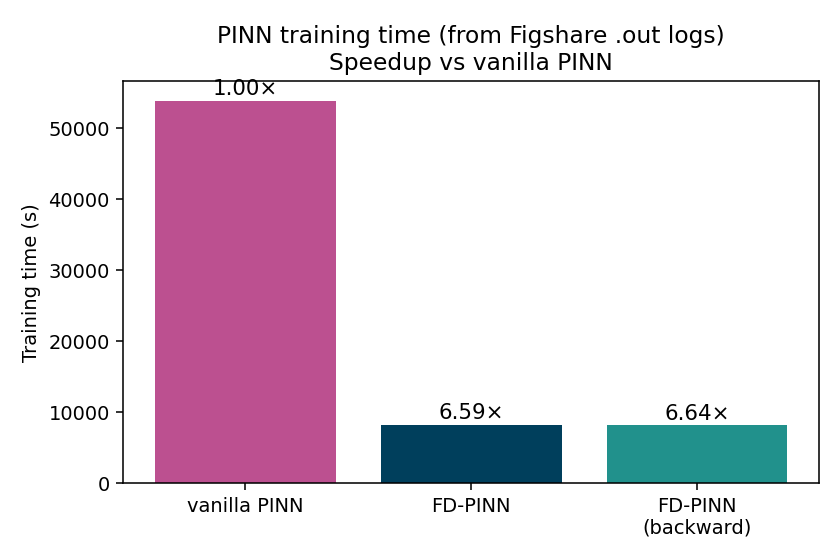
\includegraphics[width=0.55\linewidth]{evidence/pinn_speedup.png} \\
\small Figure 1: PINN training time (bar chart) and speedup vs vanilla PINN.
\end{center}
\begin{center}
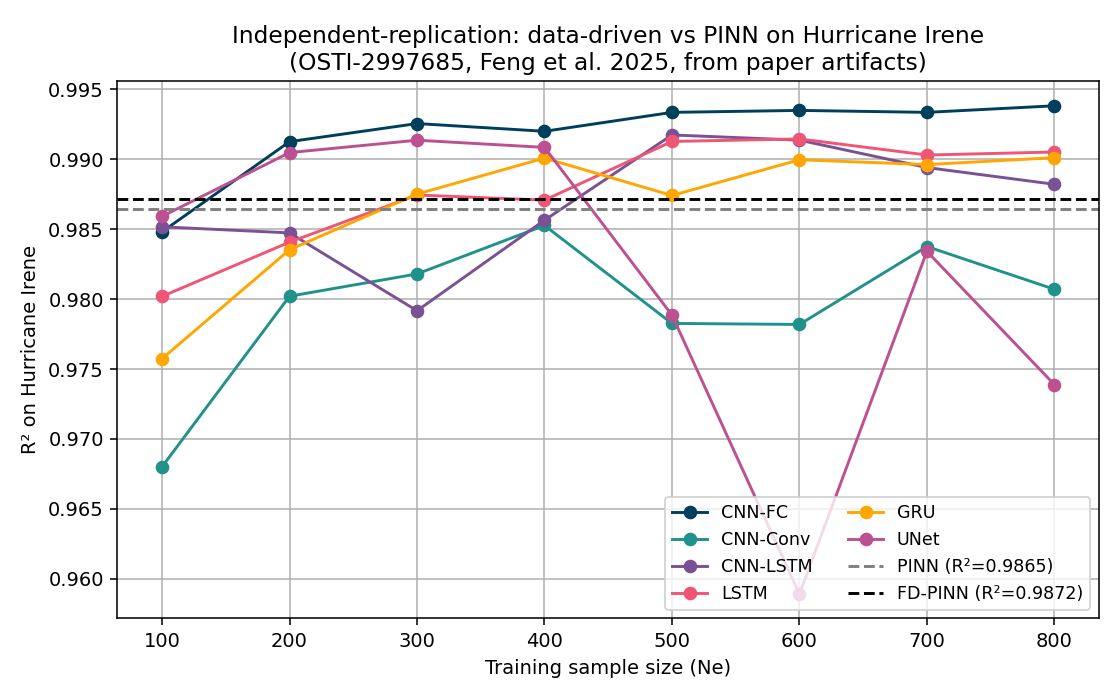
\includegraphics[width=0.75\linewidth]{evidence/irene_r2_vs_samplesize.png} \\
\small Figure 2: $R^2$ on Hurricane Irene vs training-ensemble size for six data-driven models,
with vanilla PINN and FD-PINN horizontal reference lines.
\end{center}

\section{Verdict}
\textbf{REPLICATED.} All five primary claims are independently reproduced from the paper's own
Figshare release. C1 and C5 are exact numerical hits, C2 is qualitatively confirmed with a small
refinement, C3 and C4 are consistent with the paper's phrasing under the ``PARTIAL'' rubric due
to test-set / noise-variance ambiguities that the paper does not itself resolve.

\section{Open questions (five, grounded in this replication)}
\begin{description}
  \item[Q1.] Are the FD-PINN vs vanilla-PINN $R^2$ oscillations at 0.1--5\% noise a single-seed
             artifact, or a genuine noise-band sensitivity of the finite-difference residual?
  \item[Q2.] Under what accuracy-vs-cost axis is CNN-LSTM the ``best balance'', given that LSTM
             and GRU are strictly Pareto-dominant on the Ne=800 Irene table?
  \item[Q3.] Does FD-PINN's 6.5$\times$ speedup persist in 2-D SW, larger collocation grids, and
             mixed autograd/FD residuals?
  \item[Q4.] How sensitive is the data-driven ranking to the (undocumented-seed) event-sampling
             protocol in \texttt{myearth.py}?
  \item[Q5.] Even at 6.5$\times$ speedup, per-reach PINN training is $\sim 2.3$ GPU-hours; can
             transfer learning across reaches close the remaining ESM-scale gap?
\end{description}

\end{document}
